\begin{table}[p]
   \centering
   \footnotesize
   \renewcommand{\arraystretch}{1.15}
   \begin{tabular}{@{}>{\centering\arraybackslash}m{0.3033\textwidth}>{\centering\arraybackslash}m{0.3033\textwidth}>{\centering\arraybackslash}m{0.3033\textwidth}@{}}
      \hline
      \multicolumn{3}{@{}c@{}}{%
         \begin{tabular}{@{}>{\centering\arraybackslash}m{\dimexpr0.455\textwidth+\tabcolsep\relax}>{\centering\arraybackslash}m{\dimexpr0.455\textwidth+\tabcolsep\relax}@{}}
            $G_8$ & Matriz de adyacencia \\
            \hline
            \noalign{\vspace{6pt}}
            \rule{0pt}{0pt}$\vcenter{\hbox{\resizebox{0.4\textwidth}{!}{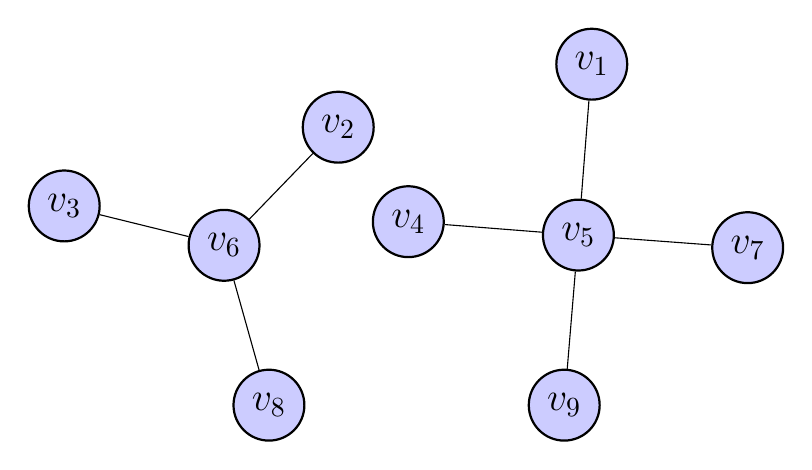
\begin{tikzpicture}[
  scale=1,
  vnode/.style={circle, fill=blue!20, draw=black, thick, minimum size=9mm, inner sep=0pt, font=\Large}
]
  % Vértices
  \node[vnode] (v1) at (7.05, 4.75) {$v_1$};
  \node[vnode] (v2) at (3.83, 3.95) {$v_2$};
  \node[vnode] (v3) at (0.35, 2.95) {$v_3$};
  \node[vnode] (v4) at (4.72, 2.75) {$v_4$};
  \node[vnode] (v5) at (6.88, 2.58) {$v_5$};
  \node[vnode] (v6) at (2.38, 2.45) {$v_6$};
  \node[vnode] (v7) at (9.03, 2.42) {$v_7$};
  \node[vnode] (v8) at (2.95, 0.42) {$v_8$};
  \node[vnode] (v9) at (6.70, 0.42) {$v_9$};

  % Aristas
  \foreach \from/\to in {v1/v5, v2/v6, v3/v6, v4/v5, v5/v7, v5/v9, v6/v8}
    \draw (\from) -- (\to);
\end{tikzpicture}
}}}$
            &
            $\vcenter{\hbox{$\displaystyle \begin{pmatrix}
         0 & 0 & 0 & 0 & 1 & 0 & 0 & 0 & 0 \\
         0 & 0 & 0 & 0 & 0 & 1 & 0 & 0 & 0 \\
         0 & 0 & 0 & 0 & 0 & 1 & 0 & 0 & 0 \\
         0 & 0 & 0 & 0 & 1 & 0 & 0 & 0 & 0 \\
         1 & 0 & 0 & 1 & 0 & 0 & 1 & 0 & 1 \\
         0 & 1 & 1 & 0 & 0 & 0 & 0 & 1 & 0 \\
         0 & 0 & 0 & 0 & 1 & 0 & 0 & 0 & 0 \\
         0 & 0 & 0 & 0 & 0 & 1 & 0 & 0 & 0 \\
         0 & 0 & 0 & 0 & 1 & 0 & 0 & 0 & 0
      \end{pmatrix}$}}$ \\
            \noalign{\vspace{6pt}}
         \end{tabular}%
      } \\
      \hline
      \multicolumn{3}{c}{\textbf{Topología de adyacencia}} \\
      \hline
      Abiertos subbásicos & Vecindades mínimas & Topología \\
      \hline
         ${A_{v_1}=\{v_5\}}$\par
         ${A_{v_2}=\{v_6\}}$\par
         ${A_{v_3}=\{v_6\}}$\par
         ${A_{v_4}=\{v_5\}}$\par
         ${A_{v_5}=\{v_1,v_4,v_7,v_9\}}$\par
         ${A_{v_6}=\{v_2,v_3,v_8\}}$\par
         ${A_{v_7}=\{v_5\}}$\par
         ${A_{v_8}=\{v_6\}}$\par
         ${A_{v_9}=\{v_5\}}$
      &
         ${U_{v_1}=\{v_1,v_4,v_7,v_9\}}$\par
         ${U_{v_2}=\{v_2,v_3,v_8\}}$\par
         ${U_{v_3}=\{v_2,v_3,v_8\}}$\par
         ${U_{v_4}=\{v_1,v_4,v_7,v_9\}}$\par
         ${U_{v_5}=\{v_5\}}$\par
         ${U_{v_6}=\{v_6\}}$\par
         ${U_{v_7}=\{v_1,v_4,v_7,v_9\}}$\par
         ${U_{v_8}=\{v_2,v_3,v_8\}}$\par
         ${U_{v_9}=\{v_1,v_4,v_7,v_9\}}$
      &
         $\{\emptyset,$ $\{v_5\},$ $\{v_6\},$ $\{v_5,v_6\},$ $\{v_2,v_3,v_8\},$ $\{v_1,v_4,v_7,v_9\},$ $\{v_2,v_3,v_5,v_8\},$ $\{v_2,v_3,v_6,v_8\},$ $\{v_1,v_4,v_5,v_7,v_9\},$ $\{v_1,v_4,v_6,v_7,v_9\},$ $\{v_2,v_3,v_5,v_6,v_8\},$ $\{v_1,\allowbreak v_4,\allowbreak v_5,\allowbreak v_6,\allowbreak v_7,\allowbreak v_9\},$ $\{v_1,\allowbreak v_2,\allowbreak v_3,\allowbreak v_4,\allowbreak v_7,\allowbreak v_8,\allowbreak v_9\},$ $\{v_1,\allowbreak v_2,\allowbreak v_3,\allowbreak v_4,\allowbreak v_5,\allowbreak v_7,\allowbreak v_8,\allowbreak v_9\},$ $\{v_1,\allowbreak v_2,\allowbreak v_3,\allowbreak v_4,\allowbreak v_6,\allowbreak v_7,\allowbreak v_8,\allowbreak v_9\},$ $\{v_1,\allowbreak v_2,\allowbreak v_3,\allowbreak v_4,\allowbreak v_5,\allowbreak v_6,\allowbreak v_7,\allowbreak v_8,\allowbreak v_9\}\}$ \\[6pt]
      \hline
      \multicolumn{3}{c}{\textbf{Topología de incidencia}} \\
      \hline
      Abiertos subbásicos & Vecindades mínimas & Topología \\
      \hline
         ${e_{1}=\{v_1,v_5\}}$\par
         ${e_{2}=\{v_2,v_6\}}$\par
         ${e_{3}=\{v_3,v_6\}}$\par
         ${e_{4}=\{v_4,v_5\}}$\par
         ${e_{5}=\{v_5,v_7\}}$\par
         ${e_{6}=\{v_5,v_9\}}$\par
         ${e_{7}=\{v_6,v_8\}}$
      &
         ${U_{v_1}=\{v_1,v_5\}}$\par
         ${U_{v_2}=\{v_2,v_6\}}$\par
         ${U_{v_3}=\{v_3,v_6\}}$\par
         ${U_{v_4}=\{v_4,v_5\}}$\par
         ${U_{v_5}=\{v_5\}}$\par
         ${U_{v_6}=\{v_6\}}$\par
         ${U_{v_7}=\{v_5,v_7\}}$\par
         ${U_{v_8}=\{v_6,v_8\}}$\par
         ${U_{v_9}=\{v_5,v_9\}}$
      &
         No discreta, con 153 abiertos \\[6pt]
      \hline
   \end{tabular}
   \caption{Topologías de adyacencia e incidencia de $G_8$}
   \label{tab:topologias_G_8}
\end{table}
